\chapter{The Simplex Method}

In Chapter~\ref{systems}, you learned how to handle systems of linear equations.
However there are many situations in which inequalities appear instead of equalities. 
In such cases we are often interested 
in an optimal solution extremizing a particular quantity of interest. 
Questions like this
are a focus of fields such as 
\href{http://en.wikipedia.org/wiki/Mathematical_optimization}{mathematical optimization}
 and 
 \href{ http://en.wikipedia.org/wiki/Operations_research}{operations research}.
For the case where the functions involved are linear,  these problems go under the
title  
\href{http://en.wikipedia.org/wiki/Linear_programming}{
{{\it linear programming}}\index{linear programming}}. Originally these ideas were driven by military applications,
but by now are ubiquitous in science and industry. Gigantic computers are dedicated to implementing linear programming methods such as
George Dantzig's 
\href{http://en.wikipedia.org/wiki/Simplex_algorithm}{simplex algorithm}--the topic of this chapter.

\section{Pablo's Problem}

Let us begin with an example. Consider again Pablo the nutritionist of problem~\ref{Pablo}, chapter~\ref{warmup}.
The Conundrum City school board has employed Pablo to design their school lunch program. Unfortunately for Pablo, 
their requirements are rather tricky:

\begin{example}(Pablo's problem)\\
The Conundrum City school board is heavily influenced by the local fruit grower's association. They have stipulated
that children eat at least 7 oranges and 5 apples per week. Parents and teachers have agreed that eating at least 15 pieces of fruit per
week is a good thing, but school janitors argue that too much fruit makes a terrible mess, so that children should eat no more than
25 pieces of fruit per week. 
\begin{center}
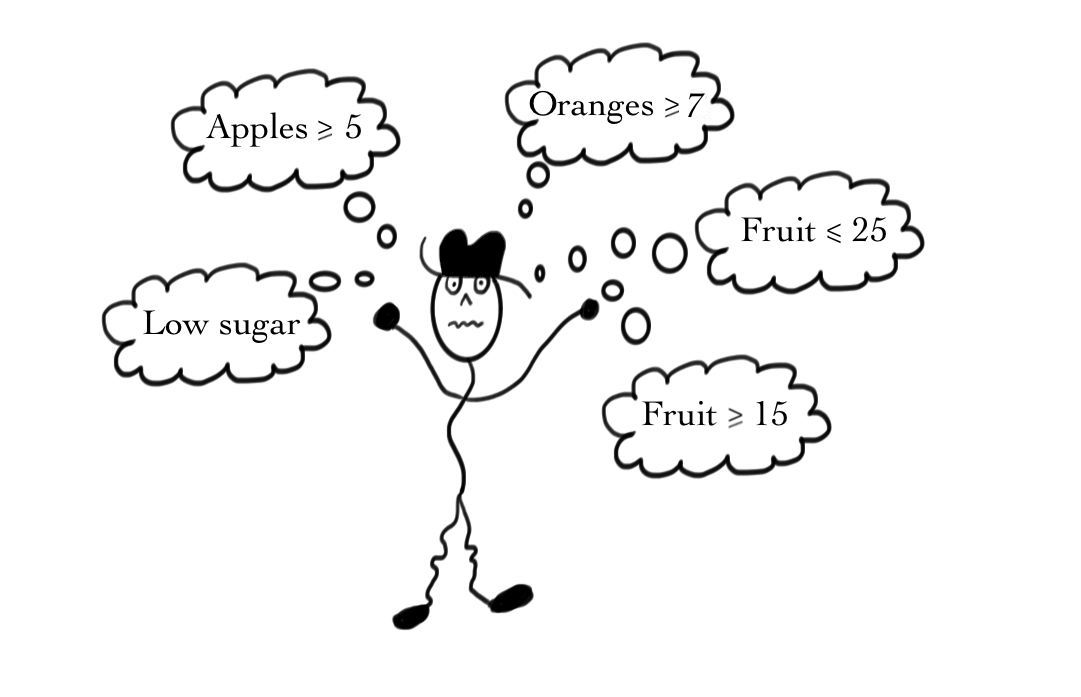
\includegraphics[scale=.3]{simplex/Pablo.jpg}
\end{center}
\noindent
Finally Pablo knows that oranges have twice as much sugar as apples
and that apples have 5 grams of sugar each. Too much sugar is unhealthy, so Pablo wants to keep the children's sugar intake as low 
as possible. How many oranges and apples should Pablo suggest that the school board put on the menu?
\end{example}

This is a rather gnarly word problem. Our first step is to restate it as mathematics, stripping away all the extraneous information:

\begin{example}(Pablo's problem restated)\\
Let $x$ be the number of apples and $y$ be the number of oranges. These must obey
$$
x\geq5\, \quad\mbox{and}\quad y\geq7\, ,
$$
to fulfill the school board's politically motivated wishes. The teacher's and parent's fruit requirement means that
$$
x+y\geq 15\, ,
$$
but to keep the canteen tidy
$$
x+y\leq 25\, .
$$
Now let 
$$s=5x+10y\, .$$
This linear function of $(x,y)$ represents the grams of sugar in $x$ apples and $y$ oranges.
The problem is asking us to minimize $s$ subject to the four linear inequalities listed above.
\end{example}

\section{Graphical Solutions}\label{graph}

Before giving a more general algorithm for handling this problem and problems like it, we note that when
the number of variables is small (preferably~2), a graphical technique can be used.

Inequalities, such as the four given in Pablo's problem, are often called {\it constraints}, and values of the variables that 
satisfy these constraints comprise the so-called {\it feasible region}. 
Since there are only two variables, this is easy to plot:

\begin{example}(Constraints and feasible region)
Pablo's constraints are
\begin{eqnarray*}
&x\geq 5&\\
&y\geq 7&\\[2mm]
&15\leq x+y\leq25\, .&
\end{eqnarray*}
Plotted in the $(x,y)$ plane, this gives:
\vspace{-5mm}
\begin{center}
\hspace{-1cm}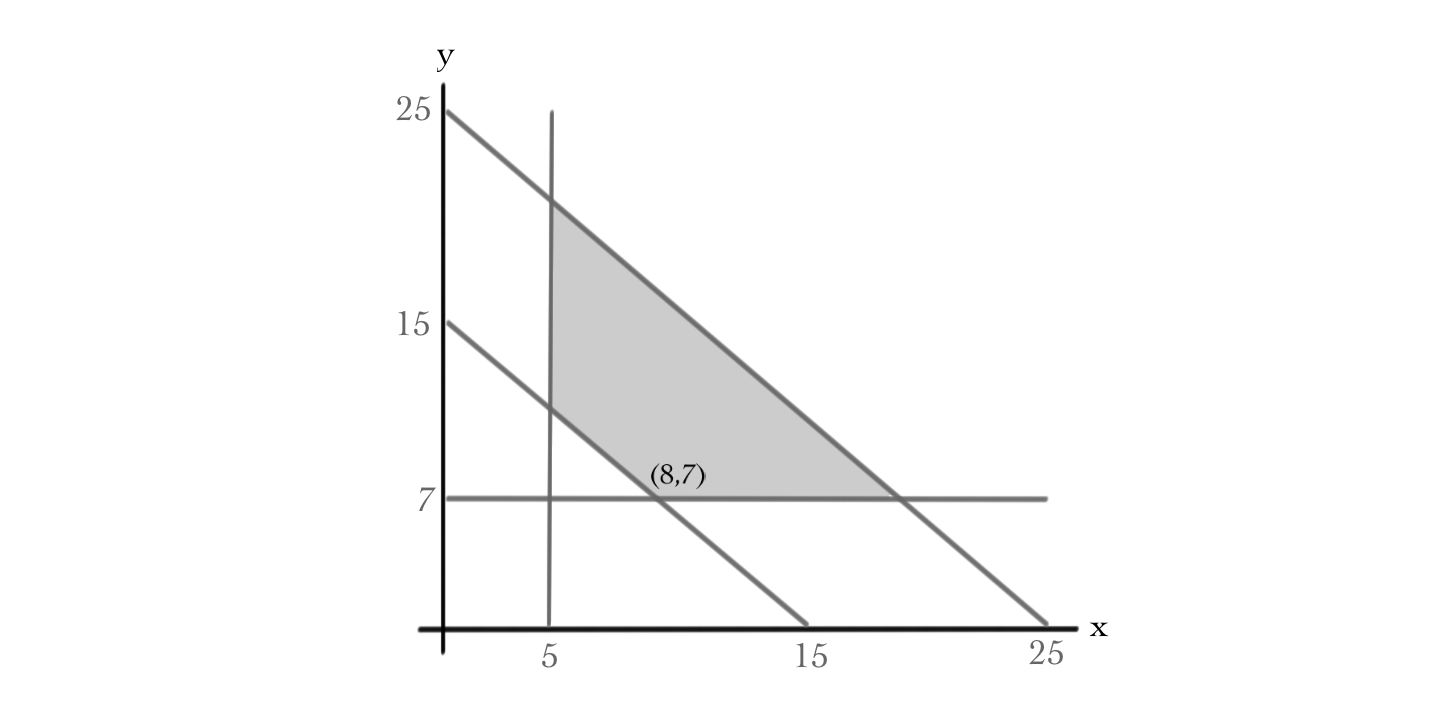
\includegraphics[scale=.32]{simplex/feasible.jpg}
\end{center}
\end{example}

You might be able to see the solution to Pablo's problem already. Oranges are very sugary, so they should be kept low, thus $y=7$.
Also, the less fruit the better, so the answer had better lie on the line $x+y=15$. Hence, the answer must be at the vertex 
$(8,7)$. Actually this is a general feature of linear programming problems, the optimal answer must lie at a vertex of the feasible region. Rather
than prove this, lets look at a plot of the linear function $s(x,y)=5x+10y$.

\begin{example}(The sugar function)\\
Plotting the sugar function requires three dimensions:
\vspace{-1.5mm}
\begin{center}
\hspace{-1cm}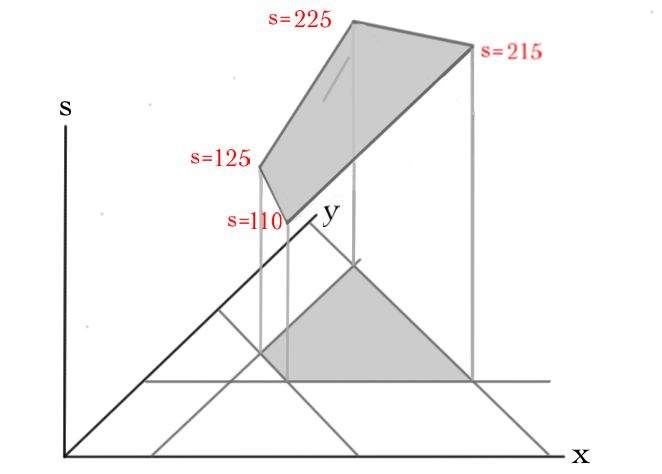
\includegraphics[scale=.38]{simplex/sugar.jpg}
\end{center}
\end{example} 

The plot of a linear function of two variables is a plane through the origin. 
Restricting the variables to the feasible region gives some lamina in 3-space.
Since the function we want to optimize is linear (and assumedly non-zero), 
if we pick a point in the middle of this lamina, we can always increase/decrease 
the function by moving out to an edge and, in turn, along that edge to a corner.
Applying this to the above picture,  we see that Pablo's best option is 110 grams of sugar a week, in the form of 
8 apples and 7 oranges.

It is worthwhile to contrast the optimization problem for a linear function with the non-linear case you may have seen in calculus courses:
\vspace{-1.5mm}
\begin{center}
\hspace{-1cm}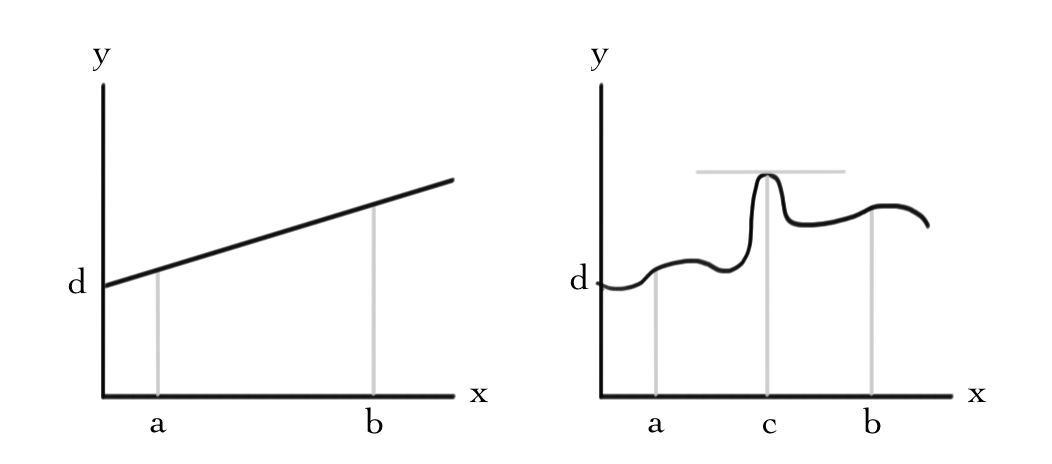
\includegraphics[scale=.33]{simplex/linvsnonlin.jpg}
\end{center}
Here we have plotted the curve $f(x)=d$ in the case where the function $f$ is linear and non-linear. 
To optimize $f$ in the interval $[a,b]$, for the linear case we just need to compute and compare the values $f(a)$ 
and $f(b)$. In contrast, for non-linear functions it is necessary to also compute the derivative $df/dx$ to study whether
there are extrema {\bf inside} the interval.

\section{Dantzig's Algorithm}\label{dantzig}

In simple situations a graphical method might suffice, but in many applications there may be thousands or even millions of variables 
and constraints. Clearly an algorithm that can be implemented on a computer is needed. The {\it simplex algorithm} (usually attributed to George Dantzig) provides exactly that. It begins with a standard problem:

\begin{problem}
Maximize $f(x_1,\ldots,x_n)$ where $f$ is linear, $x_i\geq 0$ ($i=1,\ldots, n$) subject~to  
$$
Mx = v\, ,\qquad x:=\ccolvec{x_1\\\vdots \\ x_n}\, ,
$$
where the $m\times n$ matrix $M$ and $m\times 1$ column vector $v$ are given.
\end{problem}
 
This is solved by arranging the information in an augmented matrix and then applying EROs.
To see how this works lets try an example.

\begin{example}\label{stdprob}
Maximize $f(x,y,z,w)=3x-3y-z+4w$ subject to constraints
\begin{equation*}
\begin{array}{rcccl}
c_1&:=&x+y+z+w&=&5\\[2mm]
c_2&:=&x+2y+3z+2w&=&6\, ,
\end{array}
\end{equation*}
where $x\geq0$, $y\geq0$, $z\geq0$ and $w\geq 0$.
\end{example}
  The key observation is this: Suppose we are trying to maximize $f(x_1,\ldots,x_n)$ subject to 
  a constraint $c(x_1,\ldots,x_n)=k$ for some constant $k$ ($c$ and $k$ would  be the entries of 
  $Mx$ and $v$, respectively, in the above). Then we can also try to maximize
  $$
 f(x_1,\ldots,x_n)+\alpha c(x_1,\ldots,x_n)\, 
  $$
  because this is only a constant shift $f\to f+\alpha k$. Choosing $\alpha$ carefully can lead to a simple form for the function we are extremizing.



\begin{example} (Setting up an augmented matrix):

Since we are interested in the optimum value of $f$, we treat it as an additional variable and add one further equation
$$
-3x+3y+z-4w+f=0\, .
$$
We arrange this equation and the two constraints in an augmented matrix
$$
\begin{array}{ccc}
\left(\begin{array}{rrrrr|r}
1&1&1&1&0&5\\[1mm]
1&2&3&2&0&6\\\hline
\!-3&3&1&\!\!-4&\ 1&\ 0
\end{array}\right)
\quad &\Leftrightarrow &% \quad 
\left\{
\begin{array}{lcl}
c_1&=&5\\[1mm]
c_2&=&6\\[1mm]
f&=&3x-3y-z+4w
\end{array}\right.
\end{array}.
$$
Keep in mind that the first four columns correspond to the positive variables $(x,y,z,w)$ and that
the last row has the information of the function $f$. The general case is depicted in figure~\ref{augD}.
\end{example}

\begin{figure}
\begin{center}
\begin{tabular}{ll}
\ \ $\overbrace{\phantom{VERYVERYERY}}^{\mbox{\tiny variables (incl. slack and artificial)}}$\ 
$\overbrace{\phantom{F}}^{\mbox{\tiny objective}}$&\\
$
\left(
\begin{array}{c|c}
\phantom{VERYVERYERYFATS}&\phantom{S}\\
\\
\\\hline
\\
\end{array}
\right)
$ &$\begin{array}{l} \\ \leftarrow  \mbox{constraint equations} \\[6mm] \leftarrow \mbox{objective equation}\end{array}$\\
\hspace{4.3cm}$\begin{array}{c}\uparrow\\ \mbox{objective value}\end{array}\!\!\!\!\!\!\!\!$
\end{tabular}
\end{center}
\caption{Arranging the information of an optimization problem in an augmented matrix.\label{augD}}
\end{figure}



Now the system is written as an augmented matrix where the last row encodes the objective function and the other rows the constraints. Clearly 
we can perform row operations on the constraint rows since this will not change the solutions to the constraints. 
Moreover, we can add any amount of the constraint rows to the last row,
since this just amounts to adding a constant to the function we want to extremize.

\begin{example} (Performing EROs)

We scan the last row, and notice the (most negative) coefficient $-4$. Na\"ively
you might think that this is good because this multiplies the positive variable $w$
and only helps the objective function $f=4w+\cdots$. However, what this actually means
is that the variable $w$ will large but determined by the constraints. Therefore we want to remove it 
from the objective function. We can zero out this entry by performing a row operation. For that, either of first two rows could be used. 
To decide which, we remember that the we still have to solve solve the constraints for variables that are positive. Hence we should try 
to keep the first two entries in the last column positive. Hence 
we choose the row which will add the smallest constant to $f$ when we zero out the $-4$: Look at the last column (where the values of the constraints are stored). We see that adding four times the 
first row to the last row would zero out the $-4$ entry but add $20$ to $f$, while adding two  times the second row to the last row would also zero out the $-4$ but only add $12$ to $f$. (You can follow this by watching what happens to the last entry in the last row.)
So we perform the latter row operation and obtain the following:
$$
\begin{array}{c|c}
\left(
\begin{array}{rrrrr|r}
1&1&1&1&0&5\\[1mm]
1&2&3&2&0&6\\\hline
\!-1&7&7&0&\ 1&\ 12
\end{array}\right)
\quad\quad  &\quad 
\begin{array}{rcl}
c_1&=&5\\[1mm]
c_2&=&6\\
f+2c_2&=&12+x-7y-7z\, .
\end{array}
\end{array}
$$
We do not want to undo any of our good work when we perform further row operations, so now we use the second row to zero out all other entries in the fourth column. This is achieved by subtracting half the second row from the first:
$$
\begin{array}{c|c}
\left(
\begin{array}{rrrrr|r}
\frac12&0&-\frac12&0&0&2\\[1mm]
1&2&3&2&0&6\\\hline
\!-1&7&7&0&\ 1&\ 12
\end{array}\right)
\quad\quad  &\quad 
\begin{array}{rcl}
c_1-\frac12 c_2&=&2\\[1mm]
c_2&=&6\\
f+2c_2&=&12+x-7y-7z\, .
\end{array}
\end{array}
$$
Precisely because we chose the second row to perform our row operations, all entries in the last column remain positive. This allows us to continue the algorithm.

We now repeat the above procedure: There is a $-1$ in the first column of the last row. We want to zero it out while adding as little to
$f$ as possible. This is achieved by adding twice the first row to the last row:
$$
\begin{array}{c|c}
\left(
\begin{array}{rrrrr|r}
\frac12&0&-\frac12&0&0&2\\[1mm]
1&2&3&2&0&6\\\hline
0&7&6&0&\ 1&\ 16
\end{array}\right)
\quad\quad  &\quad 
\begin{array}{rcl}
c_1-\frac12 c_2&=&2\\[1mm]
c_2&=&6\\
f+2c_2+2(c_1-\frac12 c_2)&=&16-7y-6z\, .
\end{array}
\end{array}
$$
The Dantzig algorithm terminates if all the coefficients in the last row (save perhaps for the last entry which encodes the value of the objective) are positive.
To see why we are done, lets write out what our row operations have done in terms of the function $f$ and the constraints $(c_1,c_2)$.
First we have
$$
f+2c_2+2(c_1-\frac12 c_2)=16-7y-6z
$$
with both $y$ and $z$ positive. Hence to maximize $f$ we should choose $y=0=z$. In which case we obtain our optimum value
$$
\underline{f=16\, .}
$$
Finally, we check that the constraints can be solved with $y=0=z$ and positive $(x,w)$. Indeed, they can by taking $x=2=w$.
\end{example} 

\section{Pablo Meets Dantzig} 
Oftentimes, it takes a few tricks to bring a given problem into the standard  form of example~\ref{stdprob}. In Pablo's case, this goes as follows.

\begin{example}
Pablo's variables $x$ and $y$ do not obey $x_i\geq 0$. Therefore define new variables 
$$
x_1=x-5\, , \quad x_2=y-7\, .
$$
The conditions on the fruit $15\leq x+y\leq 25$ are inequalities, 
$$
x_1+x_2\geq 3\, ,\quad x_1+x_2\leq 13\, ,
$$ 
so are not of the form $Mx = v$. To achieve this we introduce two new positive variables $x_3\geq0$, $x_4\geq 4$ and write
$$
c_1:=x_1+x_2-x_3=3\, ,\quad c_2:=x_1 + x_2 + x_4=13\, .
$$
These are called {\it slack variables} because they take up the ``slack'' required to convert inequality to equality.
This pair of equations can now be written as $Mx=v$,
$$
\begin{pmatrix}
1 &1&\!\!-1&0\\
1&1&0&1
\end{pmatrix}
\colvec{x_1\\x_2\\x_3\\x_4}=
\colvec{3\\\!13}\, .
$$
Finally, Pablo wants to minimize sugar $s=5x+10y$, but the standard problem maximizes $f$. Thus the so-called {\it objective function}
$f=-s+95=-5x_1-10x_2$. (Notice that it makes no difference whether we maximize $-s$ or $-s+95$, we choose the latter since it is
a linear function of $(x_1,x_2)$.)
Now we can build an augmented matrix whose last row reflects  the objective function equation $5 x_1+10 x_2 +f=0$:
$$
\left(\begin{array}{rrrrr|r}
1&1&-1&0&0&3\\
1&1&0&1&0&13\\\hline
5&10&\ 0&0&1&0
\end{array}\right)\, .
$$
Here it seems that the simplex algorithm already terminates because the last row only has positive coefficients, so that setting $x_1=0=x_2$
would be optimal. However, this does not solve the constraints (for positive values of the slack variables $x_3$ and $x_4$).
Thus one more (very dirty) trick is needed. We add two more, positive, (so-called) {\it artificial variables} $x_5$ and $x_6$ to the problem
which we use to shift each constraint 
$$
c_1\to c_1-x_5\, ,\qquad c_2\to c_2-x_6\, .
$$
The idea being that for large positive~$\alpha$,  the modified objective function $$f-\alpha x_5 - \alpha x_6$$
is only maximal when the artificial variables vanish so the underlying problem is unchanged. 
Lets take $\alpha=10$ (our solution will not depend on this choice) so that our augmented matrix reads 
\begin{eqnarray*}&&
\left(\begin{array}{rrrrrrr|r}
1&1&-1&0&1&0&0&3\\
1&1&0&1&0&1&0&13\\\hline
5&10&\ 0&0&10&10&1&0
\end{array}\right)\\[2mm]
&\stackrel{\small R_3'=R_3-10 R_1-10R_2 }\sim&
\left(\begin{array}{rrrrrrr|r}
1&1&-1&0&1&0&0&3\\
1&1&0&1&0&1&0&13\\\hline
\!-15&-10&\ 10&-10&0&0&1&-160
\end{array}\right)
\, .
\end{eqnarray*}
Here we performed one row operation to zero out the coefficients of the artificial variables.
Now we are ready to run the simplex algorithm exactly as in section~\ref{dantzig}. The first row operation 
uses the~$1$ in the top of the first column to zero out the most negative entry in the last row:
\begin{eqnarray*}&&
\left(\begin{array}{rrrrrrr|r}
1&1&-1&0&1&0&0&3\\
1&1&0&1&0&1&0&13\\\hline
0&5&-5&-10&15&0&1&-115
\end{array}\right)\\[2mm]
&\stackrel{\small R_2'=R_2-R_1}\sim&
\left(\begin{array}{rrrrrrr|r}
1&1&1&0&1&0&0&3\\
0&0&1&1&-1&1&0&10\\\hline
0&5&-5&-10&15&0&1&-115
\end{array}\right)\\[2mm]
&\stackrel{\small R_3'=R_3+10R_2}\sim&
\left(\begin{array}{rrrrrrr|r}
1&1&1&0&1&0&0&3\\
0&0&1&1&-1&1&0&10\\\hline
0&5&5&0&5&10&1&-15
\end{array}\right)
\, .
\end{eqnarray*}
Now the variables $(x_2,x_3,x_5,x_6)$ have zero coefficients so must be set to zero to maximize $f$.
The optimum value is $f=-15$ so $s=-f-95=110$ exactly as before. Finally, to solve the constraints $x_1=3$
and $x_4=10$ so that $x=8$ and $y=7$ which also agrees with our previous result.
 \end{example}


Clearly, performed by hand,  the simplex algorithm was slow and complex for Pablo's problem. However, the key point is
that it is an algorithm that can be fed to a computer. For problems with many variables, this method is much faster than 
simply checking all vertices as we did in section~\ref{graph}.

\section{Review Problems}

%\section{Review Problems}





\begin{enumerate}

\item Let $D=\begin{pmatrix}
\lambda_1 & \mc0 \\
\mc0 & \lambda_2 \\
\end{pmatrix}$.
\begin{enumerate}
\item Write $D$ in terms of the vectors $e_1$ and $e_2$, and their transposes.
\item Suppose $P=\begin{pmatrix}
a & b \\
c & d \\
\end{pmatrix}$ is invertible.  Show that $D$ is similar to
\[
M=\frac{1}{ad-bc}\begin{pmatrix}
\lambda_1ad-\lambda_2bc & -(\lambda_1-\lambda_2)ab \\[1mm]
(\lambda_1-\lambda_2)cd & -\lambda_1bc + \lambda_2ad
\end{pmatrix}.
\]
\item Suppose the vectors $\rowvec{a,b}$ and $\rowvec{c,d}$ are orthogonal.  What can you say about $M$ in this case? (Hint: think about what \(M^T\) is equal to.)
\end{enumerate}

\phantomnewpage

\item \label{orthogprob} Suppose $S=\{v_1, \ldots, v_n \}$ is an \emph{orthogonal} (not orthonormal) basis for~$\Re^n$.  Then we can write any vector $v$ as $v=\sum_ic^iv_i$ for some constants $c^i$.  Find a formula for the constants $c^i$ in terms of $v$ and the vectors in~$S$.

\Videoscriptlink{orthonormal_bases_hint.mp4}{Hint}{scripts_orthonormal_bases_hint}
\phantomnewpage

\item \label{orthogprojprob} Let $u,v$ be linearly independent vectors in $\Re^3$, and $P=\spa \{ u,v\}$ be the plane spanned by $u$ and $v$.  
\begin{enumerate}
\item Is the vector $v^\bot := v-\frac{u\cdot v}{u\cdot u}u$ in the plane $P$?
\item  What is the (cosine of the) angle between $v^\bot$ and $u$?
\item %Given your solution to the above, 
How can you find a third vector perpendicular to both $u$ and $v^\bot$?
\item  Construct an orthonormal basis for $\Re^3$ from $u$ and $v$.
\item  Test your abstract formul\ae\ starting with 
\[
u=\rowvec{1 , 2 , 0} \text{ and } v=\rowvec{0 , 1 , 1}.
\]
\end{enumerate}

\Videoscriptlink{orthonormal_bases_hint3.mp4}{Hint}{scripts_orthonormal_bases_hint3}

\phantomnewpage



\item Find an orthonormal  basis for $\Re^4$ which includes $(1,1,1,1)$ using the following procedure:\\
\begin{enumerate} 
\item Pick a vector perpendicular to the vector 
$$v_1 =\colvec{1\\1\\1\\1}$$ from the solution set of the matrix equation $$v_1^Tx=0\, .$$ Pick the vector $v_2$ obtained from the standard Gaussian elimination procedure which is the coefficient of $x_2$.
\item Pick a vector perpendicular to both $v_1$ and $v_2$ from the solutions set of the matrix equation $$\colvec{v_1^T\\[1mm]v_2^T}x=0\, .$$ Pick the vector $v_3$ obtained from the standard Gaussian elimination procedure with $x_3$ as the coefficient. 
\item Pick a vector perpendicular to $v_1,v_2,$ and $v_3$ from the solution set of the matrix equation $$\colvec{v_1^T\\[1mm]v_2^T\\[1mm]v_3^T}x=0\, .$$  Pick the vector $v_4$ obtained from the standard Gaussian elimination procedure with $x_3$ as the coefficient. 
\item Normalize the four vectors obtained   above.
\end{enumerate}


\item Use the inner product $$f\cdot g := \int_0^1 f(x)g(x)dx$$  on the vector space $V={\rm span} \{1,x,x^2,x^3\}$ to perform the Gram-Schmidt procedure on the set of vectors $\{1,x,x^2,x^3\}$. 

\item Use the inner product $$f\cdot g := \int_0^{2\pi} f(x)g(x)dx$$  on the vector space $V={\rm span} \{\sin(x),\sin(2x),\sin(3x) \}$ to perform the Gram-Schmidt procedure on the set of vectors $\{\sin(x),\sin(2x),\sin(3x) \}$. \\
Try to build an orthonormal basis for the vector space $$\spa \{ \sin(nx)~| ~n\in \N \}\, .$$
%What do you suspect about the vector space $\spa \{ \sin(nx)~| ~n\in \N \}$?\\
%What do you suspect about the vector space $\spa \{ \sin(ax)~|~ a \in \Re \}$?
\item 
\begin{enumerate}
\item
Show that if $Q$ is an orthogonal $n\times n$ matrix, then $$u\dotprod v = (Qu)\dotprod (Qv)\, ,$$ for any $u,v\in \Re^n$. That is, $Q$ preserves the inner product. 
\item Does $Q$ preserve the outer product? 
\item  If the set of vectors $\{ u_1,\dots,u_n\}$ is orthonormal and $\{ \lambda_1,\cdots,\lambda_n\}$ is a set of numbers, 
then what are the eigenvalues and eigenvectors of the matrix
$M=\sum_{i=1}^n \lambda_i u_i u_i^T$? 
\item How would the eigenvectors and eigenvalues of this matrix change if we replaced  $\{ u_1,\dots,u_n\}$ by $\{ Qu_1,\dots,Q u_n\}$?
\end{enumerate}


\item Carefully write out the Gram-Schmidt procedure for the set of vectors 
$$\left\{ \colvec{1\\1\\1}, \colvec{1\\-1\\1}, \colvec{1\\1\\-1} \right\} \, .$$ Is it possible to rescale the second vector obtained in the procedure to a vector with integer components? 


\item 
\label{basisortho}
\begin{enumerate}
\item Suppose $u$ and $v$ are linearly independent.  Show that $u$ and $v^\perp$ are also linearly independent.  Explain why $\{u, v^\perp\}$ is a basis for $\spa \{u,v\}$.



\Videoscriptlink{gram_schmidt_and_orthogonal_complements_hint.mp4}{Hint}{gram_schmidt_and_orthogonal_complements_hint}

\item Repeat the previous problem, but with three independent vectors $u,v,w$
 where $v^\perp$ and $w^\perp$ are as defined by the Gram-Schmidt procedure. 
\end{enumerate}

\phantomnewpage


\item \label{QRprob} Find the $QR$ factorization of
$$
M=\begin{pmatrix}1&0&\phantom{\!-}2\\-1&2&0\\-1&-2&2
\end{pmatrix}\, .
$$

\phantomnewpage

\item Given any three vectors $u,v,w$, when do $v^\perp$ or $w^\perp$ of the Gram--Schmidt procedure vanish?

\phantomnewpage

\item For $U$ a subspace of $W$, use the subspace theorem to check that $U^\perp$ is a subspace of $W$.

\phantomnewpage


\phantomnewpage

\item %(Extra Credit) 
Let $S_n$ and $A_n$ define the space of $n \times n$ symmetric and anti-symmetric matrices, respectively. These are subspaces of the vector space $M^n_n$ of all $n\times n$ matrices. What is $\dim M^n_n$, $\dim S_n$, and $\dim A_n$? Show that $M^n_n = S_n + A_n$. Define an inner product on square matrices
$$
M\cdot N ={\rm tr} MN\, .
$$
Is $A_n^{\perp}=S_n$? Is $M^n_n = S_n \oplus A_n$?

%\emph{Hint: Note that $\dim S_n = \dim U_n$ where $U_n$ is the vector space of all $n \times n$ upper triangular matrices, and also note that $\dim A_n = \dim \widetilde{U}_n$ where $\widetilde{U}_n$ is the vector space of all strictly $n \times n$ upper triangular matrices (\emph{i.e.} the diagonal entries are all 0).}

\item The vector space $V={\rm span} \{ \sin(t),\sin(2t), \sin(3t) , \sin(3t)\}$ has an inner product: 
$$f\cdot g:=\int _0^{2\pi}f(t)g(t) dt\, .$$ Find the orthogonal compliment to $U={\rm span} \{ \sin(t)+\sin(2t) \}$ in $V$. Express $\sin(t)-\sin(2t)$ as  the sum of vectors from $U$ and $U^\perp$.

\end{enumerate}

\phantomnewpage

